\section{Background and contributions}
\Gls{ibc} systems are feedback control systems whose feedback is provided by camera(s) as the sensor(s) (illustrated in Fig.~\ref{fig:ch7_ibc_intro}~(a)).
A camera captures image frames at a pre-defined constant frame rate from the dynamic system environment.
A compute-intensive image-processing algorithm processes the image frames to detect features in the image such as objects, traffic signs and lanes.
These features are then used to compute the states of the system, such as relative position and distance~\cite{corke2017robotics}.
A controller computes the control input for actuation using the computed states.
The actuation task applies the computed control input to the \gls{ibc} system.

A typical periodic implementation of such an \gls{ibc} system is illustrated in Fig.~\ref{fig:ch7_ibc_intro}~(b).
The main challenge here is to deal with the inherent long (worst-case) sensing delay due to compute-intensive image-processing algorithms.
A long processing delay results in dropping some camera frames from processing. 
Moreover, the sensing delay is variable due to image-workload variations~\cite{mohamed2019designing}. These variations can be captured statistically using a probability distribution~\cite{adyanthaya2014robustness} (illustrated in Fig.~\ref{fig:ch7_ibc_intro}~(c)).
A long worst-case sensing delay leads to a long sensor-to-actuator delay $\tau$ (the time between the start of a sensing task and the end of the corresponding actuation task) and thus results in degraded control performance~\cite{sharkey1996delays,aastrom2013computer}.
The question is: \textit{How to cope with the long variable sensing delay in an \gls{ibc} system?}

\begin{figure}[t]
\centerline{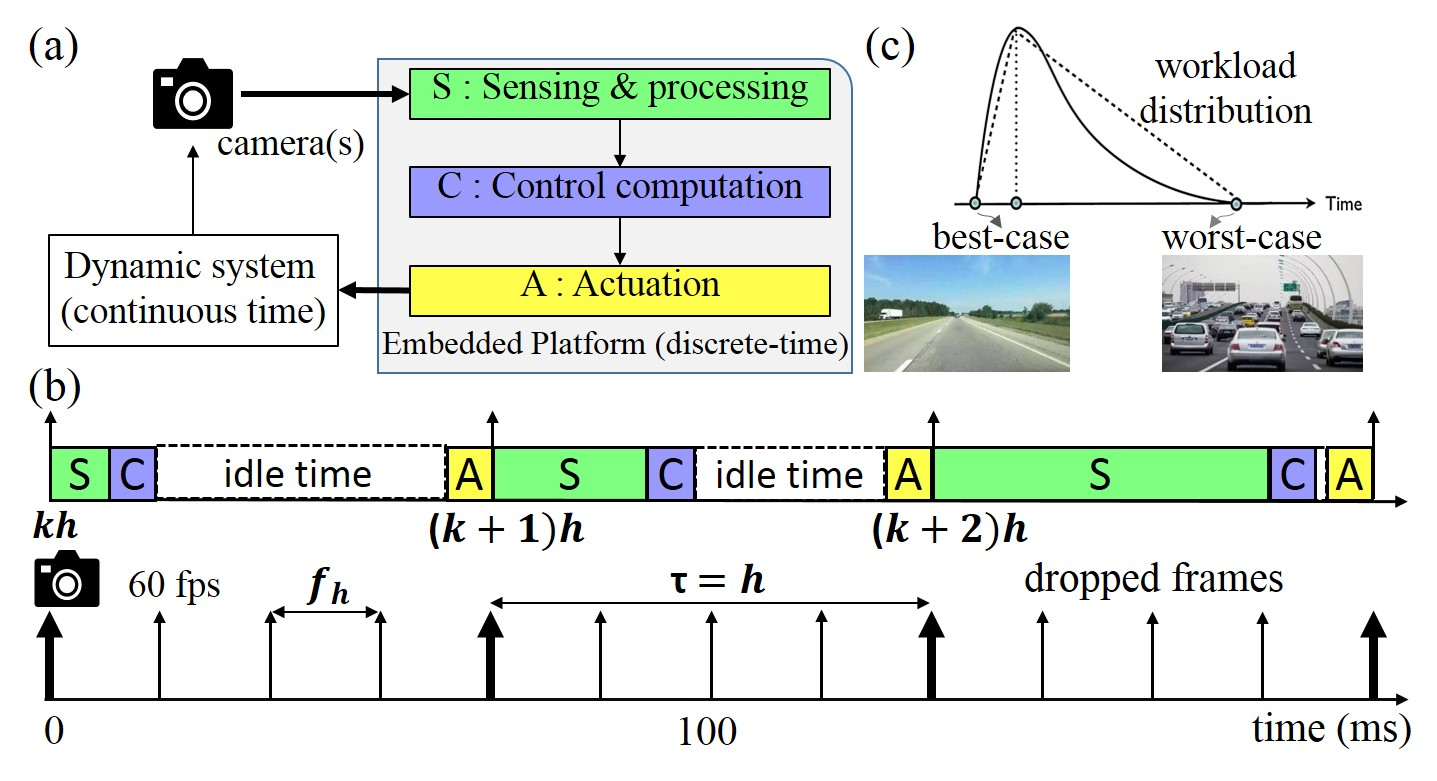
\includegraphics[width=\textwidth]{images/ibc_intro.jpg}}
\vspace{-1ex}
\caption{An \gls{ibc} system: (a) block diagram; (b) Gantt chart for a typical \gls{ibc} implementation; (c) workload variations captured as a distribution. (repeating Fig.~\ref{fig:ch1_ibc_intro}, for readability)}
\label{fig:ch7_ibc_intro}
%\vspace{-2em}
\end{figure}

\begin{figure}[t]
\centerline{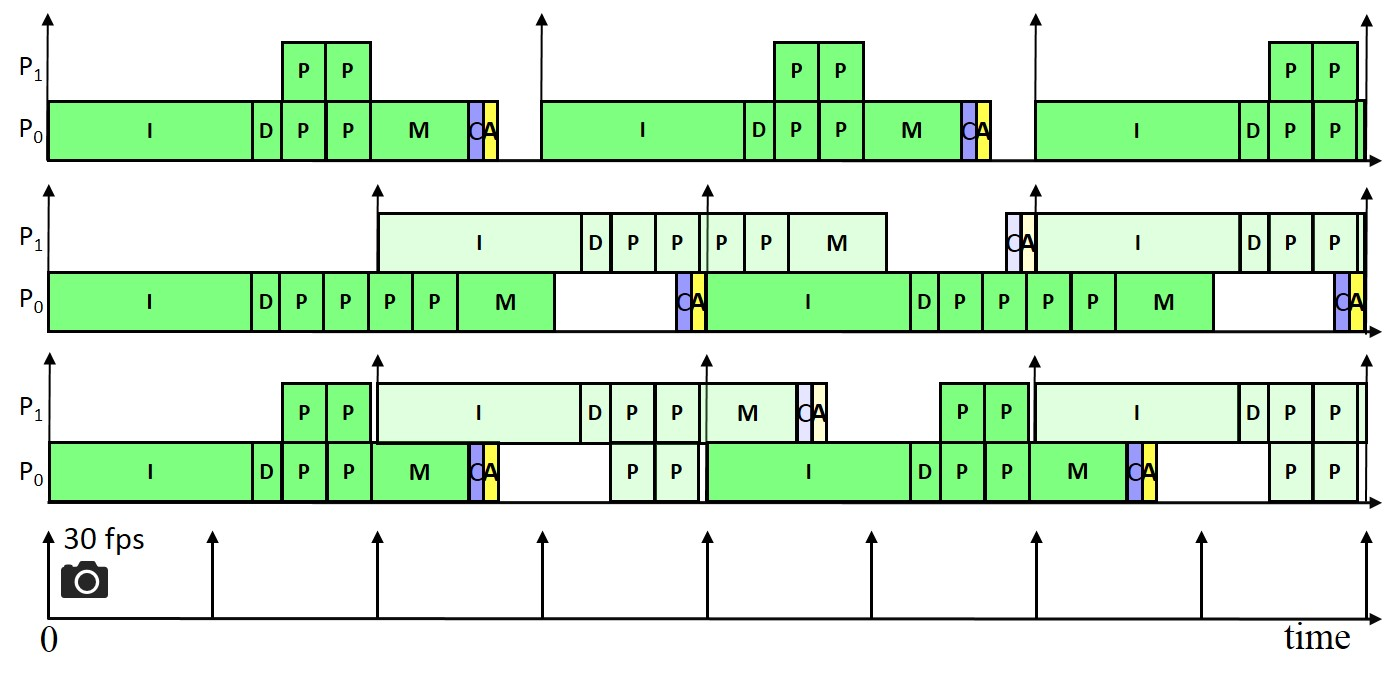
\includegraphics[width=\textwidth]{images/ibc_gantt2.jpg}}
\vspace{-1ex}
\caption{\Gls{ibc} implementations for worst-case image workload: (a) Parallelisation of sensing; (b) Pipelining without resource sharing; (c) Pipelining and parallelism together with resource sharing. 
Note: 1) Sensing task \taskS~is composed of image signal (pre-)processing (\taskISP), \gls{roi} detection \taskRoID, \gls{roi} processing \taskRoIP, and \gls{roi} merging \taskRoIM explained in Section~\ref{sec:ch7_IBCGraph}; 2) \processor$_0$ and \processor$_1$ are the two processing cores.}
\label{fig:ch7_ibc_gantt}
%\vspace{-2em}
\end{figure}

The advent of multiprocessor platforms enables \textbf{coping with the long sensing delay} by either \textit{parallelising the sensing task} (explained in Chapter~\ref{chap:parallelisation}) or \textit{pipelining the control loop}~\cite{krautgartner1998performance,medina2019designing}.
Parallelisation refers to executing sensing subtasks in parallel and thereby reduces the delay compared to the worst case (illustrated in Fig.~\ref{fig:ch7_ibc_gantt}~(a)).
It is, however, limited by the degree of parallelism of the sensing algorithm.
Pipelining refers to the pipelined execution of the control loop over multiple processing cores. 
Pipelining helps to reduce the number of camera frames being skipped. It reduces the sampling period $h$ (the time between the start of two successive sensing tasks) by processing frames on available cores (illustrated in Fig.~\ref{fig:ch7_ibc_gantt}~(b)).
Pipelining is, however, limited by the presence of inter-frame dependencies, i.e., the data or algorithmic dependencies between consecutive frame processing, e.g., due to video coding~\cite{li2015lagrangian} or visual tracking~\cite{smeulders2013visual}.
In literature, the controller implemented for the pipelining is for $\tau > h$~\cite{krautgartner1998performance,medina2019designing} and for parallelisation is for $\tau\le h$~\cite{mohamed2018optimising,mohamed2020scenario} (and Chapter \ref{chap:parallelisation} of this thesis).
\vspace{1mm}

\noindent\textbf{Why should we consider pipelining and parallelism together?}
Pipelining does not reduce the delay $\tau$ compared to the worst case. By executing the frames in a pipeline, only $h$ is reduced, whereas parallelising the sensing tasks reduces $\tau$. 
However, $h$ is still at least $\tau$ for a parallel implementation. 
Considering both pipelining and parallelism together helps to reduce both $\tau$ and $h$ and thereby improves the \gls{qoc} of our \gls{ibc} system.
Further, the inherent limitations of pipelining - due to inter-frame dependencies - and parallelism - due to a limited degree of parallelism of the algorithm~- can be mitigated significantly by considering them both together.
The challenge then is to identify the optimal implementation choice considering both the degrees of pipelining and parallelism that improves the system performance.
The degree of pipelining is quantified by the maximum number of active pipes in the pipeline, and the degree of application parallelism is quantified by the maximum amount of parallel execution within one sensing task.
Both are limited by the available processing resources.
\vspace{1mm}

\noindent\textbf{Challenges:}
The literature prior to this work does not explore the impact of both pipelining and parallelism together on the \gls{qoc} of \gls{ibc} implementation.
Existing pipelined \gls{ibc} implementations ~\cite{krautgartner1998performance,medina2019designing} assume that the mapping is given, and that each pipe is mapped to a unique resource \textit{without any resource sharing between pipes}. This is a restrictive implementation choice. Inter-frame dependencies, which are crucial for practical implementation, are also not considered. We considered inter-frame dependencies in the previous chapter, and consider them integrally in combination with parallelisation in this chapter.
There are two main challenges that were not explicitly explored prior to this work.
First, how to model a multiprocessor \gls{ibc} system considering both pipelining and parallelism together? 
The challenge in modelling is to explicitly consider workload variations, inter-frame dependencies and constant (often periodic) control timing parameters $\tau$ and $h$.
Second, how to identify the optimal mapping of the sensing task on shared processing resources that considers both pipelining and parallelism together and provides a tight analytical bound on control timing parameters $\tau$ and $h$ so as to optimise \gls{qoc}.

As already motivated, we chose \gls{sadf}~\cite{theelen2006scenario} as our \gls{moc} as it inherently supports modelling scenarios and has tool support for timing analysis and platform-aware mapping.
Existing mapping analysis tools~\cite{stuijk2006sdf,anssi2012chronval} typically assume that each node (subtask or actor) in the graph is bound to one processing resource. Pipelining involves (possibly) concurrent executions of subtasks on multiple resources, with inter-frame dependencies between actor instances. Moreover, control assumes careful time-triggered execution of sensing and actuation tasks. All these aspects can only be analysed after non-trivial graph transformations (as e.g.\ exemplified in~\cite{lattuada2013modeling}).

Fig.~\ref{fig:ch7_ibc_gantt}~(c) illustrates an implementation of two pipes on a shared platform allocation of two processors, with each pipe having a parallelised sensing subtask. 
With parallelised pipes but without resource sharing between pipes, we would need four processors to achieve the same delay and period as obtained in Fig.~\ref{fig:ch7_ibc_gantt}~(c).
To integrally consider pipelining and parallelisation on a shared multiprocessor platform, we need an efficient analysis to identify the optimal mapping. The mapping should guarantee the required (often constant) worst-case delay and period for the controller design. 

\vspace{1mm}

\noindent \textbf{The contributions} of this chapter are as follows:
\begin{enumerate}
\item We extend the \gls{spade} approach, presented in Chapters \ref{chap:parallelisation}, by considering pipelining of the control loop and formalising the \gls{ibc} system modelling. This complete version of the \gls{spade} approach (as explained in Section~\ref{sec:ch7_designFlow}) integrally considers pipelining and parallelism for a multiprocessor \gls{ibc} implementation. 
The exact problem addressed is the following: \textit{For a given multiprocessor platform allocation, identify the optimal design choice for an \gls{ibc} system considering both pipelining and parallelism and explicitly considering image-workload variations, inter-frame dependencies, resource sharing between pipes and platform constraints.}
    The optimal design choice identifies the degree of pipelining and degree of parallelism required for maximising the \gls{qoc} and is translated into \textit{system configurations} that guarantee control timing parameters.
    \item We propose model transformations for modelling, analysing, and mapping the \gls{ibc} system. 
The model transformations for pipelined parallelism  are the main contribution. These transformations consider both pipelining and parallelism together (as explained in Section~\ref{sec:ch7_ModelTransformations}). 
    The model transformations allow us to relate the dataflow timing (throughput and latency) analysis to the key control timing parameters ($h$ and $\tau$) and to optimise the mapping while integrally considering pipelining and parallelism along with workload variations, inter-frame dependencies and resource-sharing between pipes.
    Implementation-aware model transformations for model-based design of \gls{ibc} systems are not considered in prior literature.
    \item We validate our approach using Matlab simulations considering a predictable multiprocessor platform - \gls{compsoc}~\cite{hansson2009compsoc} - and using \gls{hil} experiments with an industrial heterogeneous multiprocessor platform - NVIDIA AGX Xavier - considering a \gls{lkas}. Both platforms and the \gls{lkas} case study were already introduced in Chapter \ref{chap:intro}. 
\end{enumerate}

The rest of the chapter is organised as follows.
Section~\ref{sec:ch7_embeddedIBC} describes the multiprocessor \gls{ibc} system implementation and the \gls{qoc} metrics.
Section~\ref{sec:ch7_designFlow} details the \gls{spade} design flow.
Section~\ref{sec:ch7_ModelTransformations} introduces the model transformations required for the \gls{spade} design flow to analyse pipelined parallelism.
Section~\ref{sec:ch7_SPADeRevisited} revisits the \gls{spade} design flow and precisely describes an algorithm using the model transformations and other considerations for pipelined parallelism.
Section~\ref{sec:ch7_ExperimentalResults} explores the experimental results, the \gls{dse}, and compares \gls{spade} with the state-of-the-art multiprocessor \gls{ibc} system implementations.
Section~\ref{sec:ch7_SPADeIndustrial} presents the \gls{spade} adaptation for an industrial platform, the NVIDIA AGX Xavier, and validates the results of our approach in a \gls{hil} setting.
Section~\ref{sec:ch7_conclusion} concludes the work and suggests possible future directions.